\subsubsection{Definition}

A two-dimensional homogeneous aquifer is chosen to verify advective dispersive transport. The dimension of the model domain is 100 $m$ by 60 $m$ where the uniform velocity field is held constant in the $x$ direction (Fig.~\ref{ModelSchematic}).

\begin{figure}[htbp!]
\centering
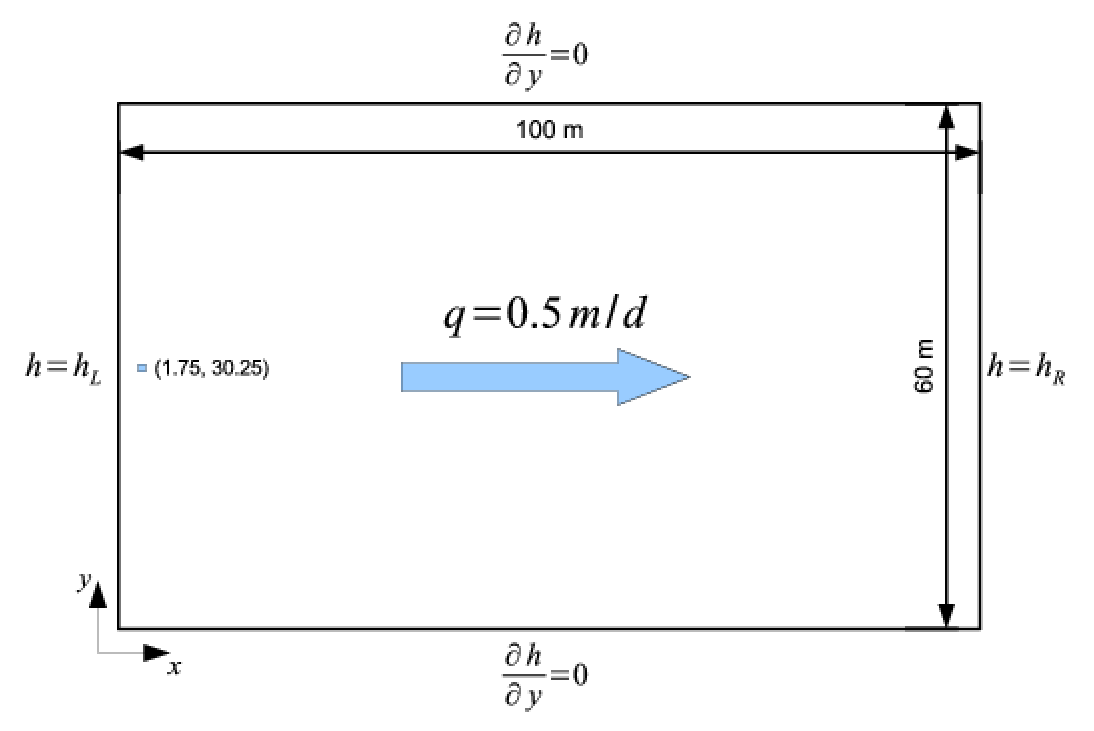
\includegraphics[scale=0.45]{PART_II/C/ModelSchematic.eps}
\caption{Particle tracking in 2D homogeneous aquifer}
\label{ModelSchematic}
\end{figure}

\subsubsection{Analytical solution}

The stated problem can be solved with an analytical solution provided by \cite{aO61}.
\begin{equation}\label{ogata}
C\left( {x,y,t} \right) = \frac{{C_0 A}}{{4\pi t\sqrt {D_{xx} + D_{yy} } }}\exp\left[ { - \frac{{\left( {x - x_0 } \right)^2 }}{{4D_{xx} t}} - \frac{{\left( {y - y_0 } \right)^2 }}{{4D_{yy} t}}} \right]
\end{equation}

where $C_0$ is the initial concentration.

\subsubsection{Numerical solution}

The domain is discretized with quadrilateral elements of 0.5 $m$ by 0.5 $m$. The same grid density is also used for converting particle distributions to element concentrations. The head gradient of one in the $x$ direction is set by assigning two constant boundary conditions along both left and right sides, thus obtains the uniform velocity field with the value of 0.5 $md^{-1}$.

The initial source load is applied to an area with dimensions of 0.1 $m$ by 0.1 $m$ to have an initial concentration of $C _0=1$ $kg m^{-3}$. The material properties for this model setup are given in Tab.~\ref{tab-2dhomo}.

\begin{table}[htbp!]
\caption{\label{tab-2dhomo}Material properties}
\begin{center}
\begin{tabular}{llrr}
\toprule
Symbol & Parameter & Value & Unit \\
\midrule
$k$ & Permeability & $1.114^{-11}$ & m$^{2}$ \\			
$\alpha _L$	   & Longitudinal dispersivity & 0.1 & m \\
$\alpha _T$	   & Transverse dispersivity & 0.1 & m \\
\bottomrule
\end{tabular}
\end{center}
\end{table}

\subsubsection{Results}

The comparison with the analytical solution is provided in Fig.~\ref{TransportHomo50K}. The number of particles used for this simulation is 50000. This is significantly less than the number of particles reported by \cite{aH03}, who reported that up to 2.5 million particles were necessary to achieve smoothness of the solution due to oscillations around the contours. As the oscillations observed here for the method proposed are smaller than reported by \cite{aH03}, the proposed method allows to dramatically reduce the number of particles required for a smooth solution by about two orders of magnitude.

\begin{figure}[htbp!]
\centering
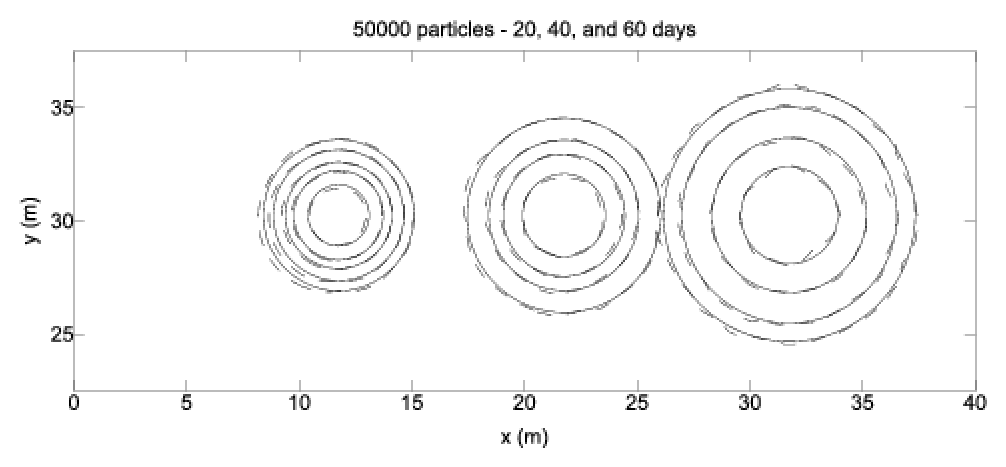
\includegraphics[scale=0.60]{PART_II/C/TransportHomo50K.eps}
\caption{Transport results of the RWPT method compared with the
analytical solution for 50000 particles at 20, 40,
and 60 days: The solid line is the analytical solution, the dotted
line is the RWPT result. Contour lines are shown for $C=2.6e^{-4}$, $1.6e^{-4}$, $1.0e^{-4}$, and $4e^{-5}$.} 
\label{TransportHomo50K}
\end{figure}

In addition, various numbers of particles used to solve the same problem produces particle clouds are shown in Fig.~\ref{ParticleClouds}.

\begin{figure}[htbp!]
\centering
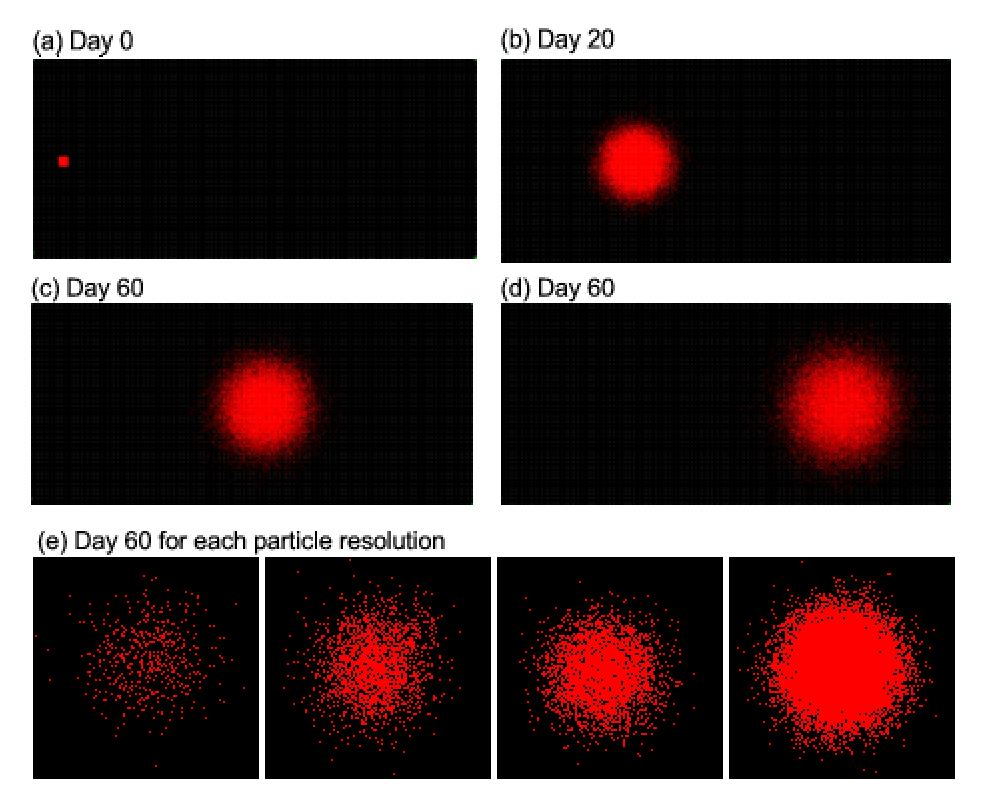
\includegraphics[scale=0.60]{PART_II/C/ParticleClouds.eps}
\caption{(a-d)Particle clouds of 50000 particles at 0, 20, 40, and 60 days, (e) Particle clouds of 1000, 5000, 10000, and 50000 particles at 60 days}
\label{ParticleClouds}
\end{figure}
